%The executive summary is a special chapter before the TOC
% See the other sections (e.g. Context) for more normal chapter headings
%%%%%%%%%%%%%%%%%%%%%%%%%%%%%%%%%%%%
% Call it Front Matter in TOC, as it will include Glossary and auto-generated TOC, LOF.
\chapter[Front Matter]{Front Matter}
\label{cha:front}
\addcontentsline{toc}{section}{Executive Summary}
%%%%%%%%%%%%%%%%%%%%%%%%%%%%%%%%%%%%
%Begin the actual executive summary text. If you create any subsections you
%probably want to use  \section*{Section name}  with an asterisk, so they are not numbered.
% Note: to get proper looking quotes use two left/right single quotes: ``. . . ''

%Example of a remark that can be optionally printed:In a world that is dynamic in almost every aspect, mobility is a necessity.  However, for persons that suffer from disabilities, their mobility may be limited.  Traveling with limited mobility can be a very difficult and burdening task especially if the travelling involves being within the small confines of an airplane.  Passengers that are faced with limited mobility or a disability have a different and often times worse experience than the average passenger during the entire flight experience.  How can have all passengers have the same experience? Designing a new futuristic cabin and creating a new travel system are essential for achieving the same experience for all passengers and to give passengers with limited mobility independence and control.

Embraer, the Brazilian airline manufacturer, decided to partner with Stanford University and the University of Sao Paulo to approach this problem of improving the entire air travel experience for persons with limited mobility or disabilities. The team from Stanford University is composed of two students and the university of Sao Paulo team is composed of 4 students, all with engineering degrees.  In collaboration, we started this journey toward a solution through extensive needfinding and benchmarking.  The needfinding centered on conducting user interviews for both the disabled passenger and the flight crew while benchmarking focused on analogous situations, patents, regulations, and current concepts and solutions.

The research that was conducted during needfinding and benchmarking was instrumental in the approach we are taking toward a solution.  The user interviews led us to the five themes we need to address with our future solution.  These themes are customer service, control, independence, seat preferences, and non-discriminatory. Figure 1 1 shows the themes and how they each rely on the others to be successful.  The interviews with potential users revealed horror stories that dealt with customer service or the lack thereof.  The solution space needs to create an environment that limits the interaction between the flight crew and the passenger to prevent these horror stories from becoming a reality for future travelers.   Independence and control were also instrumental in our findings.  The users of our solution want to feel independent and in control of their situation even though they might need assistance.  This leads our solution path to one that centers on automation and allowing the user to control their surroundings instead of the other way around.  One major discovery we made concerned the seat that a person with limited mobility chose when boarding the flight.  They chose to sit in the window seat instead of the easier-to-access aisle seat to accommodate other passengers, not themselves.  This brought us to the idea of making every seat accessible for all passengers regardless of mobility status.  The final theme motivating our solution is a non-discriminatory design.  Limited mobility passengers and passengers with disabilities have a condition that singles them out to begin with so why should our design add insult to injury by singling them out more?  Therefore, we are focusing on a universal design that would aid and improve the experience for both the limited mobility passenger and the average passenger.

These themes were our driving forces for the critical function and critical experience prototypes we created to further explore our problem space.  The team created a number of prototypes but really focused on the ones that solved this problem; one being a more incremental fix while the other addressed a more futuristic cabin.  The incremental fix was a swivel chair that would address the window versus aisle debate in the Embraer cabins with rows of 2 seats.  But what if we wanted to apply our solution to larger cabins? We then looked at a more futuristic design, which came in the CFP of seats of rails. Figure 1 2 shows the concept of the seats on rails in a clay mock-up. Here, the rows will move forward and back to provide a certain row with extra room to allow a passenger to get in and out without disturbing the other passengers.  This concept brought light to all the solutions that could be implemented and what we could make the design space to be.

\begin{figure}[h]
  \centering
     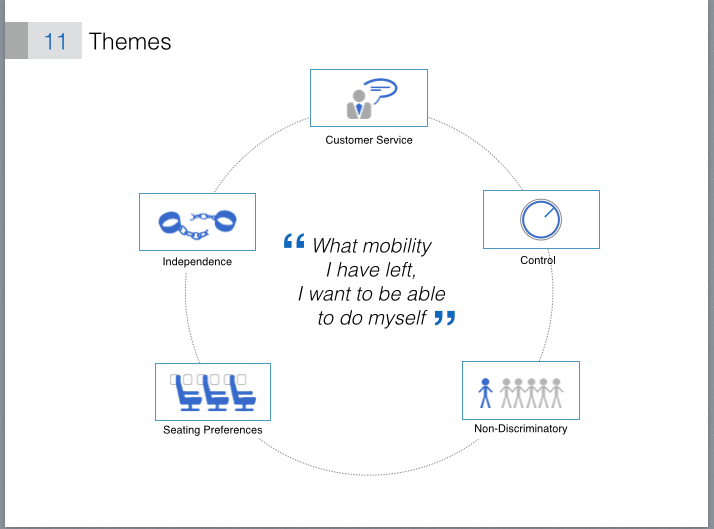
\includegraphics[width=7cm]{images/image007.png}
   \caption{Main themes driving our solution}
  \label{fig:main_themes}
\end{figure}

Our vision for a solution is a more dynamic cabin that allows the user to customize the space to his needs and allows for a more enjoyable and interactive experience.  If the world we live in is dynamic, then why does the airplane cabin have to be static with the same seating arrangements in all planes?  This is what we want to change.  We want to change the way a passenger looks at the flying experience and how they feel before, during, and after the flight.  The passengers should have more control over the seat selection, the firmness/softness of their seat, the angle, and the orientation; this list is endless. Giving passengers more independence and control while minimizing customer service interaction and discrimination is our motivation for a futuristic cabin that will make the entire air travel experience from home to gate to destination out of this world.

\begin{figure}[h]
  \centering
     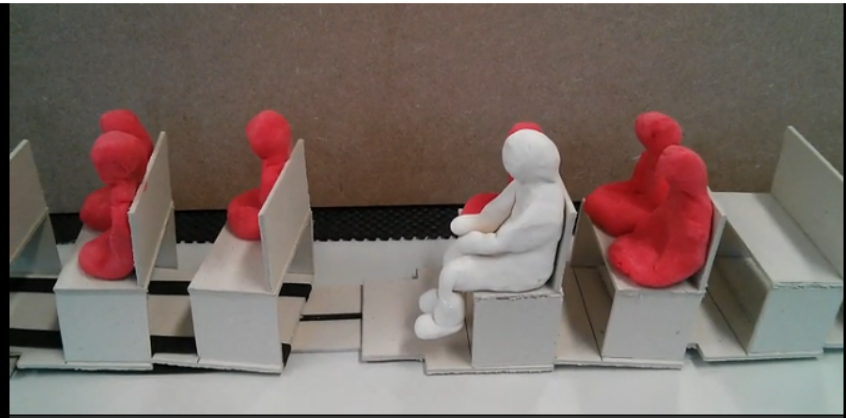
\includegraphics[width=7cm]{images/image008.png}
   \caption{Scaled mock-up of seats on rails prototype}
  \label{fig:mock_up_on_rails}
\end{figure}


%\section*{Glossary}

%\begin{list}{-}{}

%\end{list}

% Set up the Glossary. The template is looking for a file called
% "glossaryterms.tex" with glossary terms and definitions.
% You can either edit this file manually or you
% can use the Memoir glossary feature in which you insert items like
%   \glossary{glossary term}{our definition of what the term means}
% wherever you like, as you write your documentation.
% When you run the report through Latex, it will create a ".glo" file like
% "OurFallDocument.glo" which you can edit to create the file "glossaryterms.tex"
% There is also perl script I made which will do the formatting for you. 
%  perl Glo2Tex OurFallDocument.glo > glossaryterms.tex

\newpage
\section*{Glossary}
\addcontentsline{toc}{section}{Glossary}
\label{sec-glossary}
\begin{description}
\begin{document}
\begin{list}
  \item  \textbf{ADA:} Americans with Disabilities Act; one of America's most comprehensive pieces of civil rights legislation that prohibits discrimination against and guarantees people with disabilities have the same opportunities as everyone else to participate in the mainstream of American life.
  \item  \textbf{Assistive Technology:} Assistive, adaptive, and rehabilitative devices for people with disabilities; promotes greater independence by enabling people to perform tasks that they were formerly unable to accomplish, or had great difficulty accomplishing.
  \item  \textbf{Benchmarking:} A standard by which something can be measured or judged.
  \item  \textbf{CEP:} Otherwise known as a Critical Experience Prototype, this is a physical prototype created to make an experience ��real enough�� to gather insights and understanding about the user’s experience.
  \item  \textbf{CFP:} Otherwise known as a Critical Function Prototype, this is a physical prototype built to test a concept that is critical to addressing the problem statement.
  \item \textbf{Control:} The power to influence or direct either people's behavior or the course of events.
  \item \textbf{Dark Horse Prototype:} A device created during the winter quarter of ME310 that was ruled out in the fall quarter or undiscovered due to being too risky or too difficult to complete��; emphasizes creative out-of-the-box thinking and exploring all of the design space for the project. 
  \item \textbf{Disability:} A physical or mental condition that limits a person's movements, senses, or activities.
  \item \textbf{FAA:} Federal Aviation Administration; United States national aviation authority whose mission is to provide the safest, most efficient aerospace system in the world, oversees all aspects of American civil aviation.
  \item \textbf{Herrmann Brain Dominance Instrument (HDBI):} Illustrates and explains the way a person prefers to think, learn, communicate and make decisions. It identifies the preferred approach to emotional, analytical, structural, and strategic thinking.
  \item \textbf{Independence:} Freedom from outside control or support.
  \item \textbf{Limited Mobility:} Mobility impairment may be caused by a number of factors, such as disease, an accident, or a congenital disorder and may be the result from neuro-muscular or orthopedic impairments. It may include conditions such as spinal cord injury, paralysis, muscular dystrophy and cerebral palsy. It may be combined with other problems as well (i.e. brain injury, learning disability, hearing or visual impairment).
  \item \textbf{Needfinding:} Discovering opportunities by recognizing the gaps in the system or the needs.
  \item \textbf{Non-Discriminatory:} Fairness in treating people without prejudice.
  \item \textbf{Pain Points:} A level of difficulty sufficient to motivate someone to seek a solution or an alternative; a problem or difficulty.
  \item \textbf{Perspective:} A particular attitude toward or way of regarding something; a point of view.
  \item \textbf{Self-Image:} The idea one has of one's abilities, appearance, and personality
  \item \textbf{ANAC:} Agencia Nacional de Aviação Civil – Brazilian National Agency of Civil Aviation
  \item \textbf{Libras:} Brazilian Sign Language
\end{list}
\end{document}   % input the list "glossaryterms.tex"
\end{description}

%%%%%% Example of an optionally printed "remark"
%\begin{remark}
%\color{blue}
%It's a sign of a successful team that the glossary becomes extensive. Define any non-obvious or invented terms. For %example, if you reference something by an acronym, that might be a glossary term. Teams also coin terms to describe %design features. Define such terms here.  Don't define obvious stuff (axle, keyboard).  

%See comments in me310report.tex if you want to generate a glossary semi-automatically from tagged keywords.
%\normalcolor
%\end{remark}

%%%%%%%%%%%%%%%%%%%%%%%%
% TOC and LOF are automatically generated -- Note that sometimes have to "compile" Latex THREE
% times to update the main .aux files, the TOC etc. files, and finally the PDF output with all changes
% propagated to the printout.
% Make Table of Contents title smaller than a normal Chapter heading:
\renewcommand{\chaptitlefont}{\normalfont\Large\bfseries}
\newpage
\tableofcontents %asterisk to prevent it from getting a number

% Optional Lists of Figures and Tables:
\newpage
\listoffigures  %Note that for this you probably want to add the [short-headings] to captions.
%\listoftables  %I decided to omit the LOT in this example.

%Back to normal size for subsequent sections
\renewcommand{\chaptitlefont}{\normalfont\Huge\bfseries}
%%%%%%%%%%%%%%%%%%%%%%%%

